\documentclass[a4paper,11pt,twocolumn]{article}
\usepackage[utf8]{inputenc}
\usepackage{t1enc}
\usepackage[icelandic]{babel}
\usepackage{graphicx}
\usepackage{latexsym}
\usepackage{fancyhdr}
\usepackage{enumerate}
\usepackage{mdwlist}
\usepackage{xcolor}
\usepackage{listings}
\usepackage{caption}
\usepackage{amsmath}
\usepackage{color}
\usepackage{courier}
\usepackage{siunitx}
\usepackage{multirow}
\usepackage[]{algorithm2e}
\newenvironment{Figure}
  {\par\medskip\noindent\minipage{\linewidth}}
  {\endminipage\par\medskip}

\newcommand{\HRule}{\rule{\linewidth}{0.5mm}}
\def\lf{\left\lfloor}   
\def\rf{\right\rfloor}
\def\lc{\left\lceil}   
\def\rc{\right\rceil}

\sloppy


\lstset{ 
language=Java,              	% choose the language of the code
basicstyle=\footnotesize,       % the size of the fonts that are used for the code
numbers=left,                   % where to put the line-numbers
numberstyle=\footnotesize,      % the size of the fonts that are used for the line-numbers
stepnumber=1,                   % the step between two line-numbers. If it is 1 each line will be numbered
numbersep=5pt,                  % how far the line-numbers are from the code
backgroundcolor=\color{white},  % choose the background color. You must add \usepackage{color}
showspaces=false,               % show spaces adding particular underscores
showstringspaces=false,         % underline spaces within strings
showtabs=false,                 % show tabs within strings adding particular underscores
frame=single,        	  		% adds a frame around the code
tabsize=2,       			  	% sets default tabsize to 2 spaces
captionpos=b,     		      	% sets the caption-position to bottom
breaklines=true,    	    	% sets automatic line breaking
breakatwhitespace=false,    	% sets if automatic breaks should only happen at whitespace
escapeinside={\%*}{*)},         % if you want to add a comment within your code
basicstyle=\footnotesize\ttfamily,
keywordstyle=\bfseries\color{green!40!black},
commentstyle=\itshape\color{purple!40!black},
identifierstyle=\color{blue},
stringstyle=\color{orange},
texcl=true,
}

\onecolumn
\setlength{\parskip}{8pt plus 1pt minus 1pt}

\begin{document}
	
	
	\newcommand*{\titleGP}{\begingroup % Create the command for including the title page in the document
	\centering % Center all text
    \begin{flushleft}
    \textsc{TÖV501M Hönnun tölva}
    
    \noindent
    \small
    Halldór Eldjárn - \emph{hae28@hi.is}\\
	Kristján Eldjárn Hjörleifsson - \emph{keh4@hi.is}
	\end{flushleft}
	\vspace*{\baselineskip} % White space at the top of the page

	\rule{\textwidth}{1.6pt}\vspace*{-\baselineskip}\vspace*{2pt} % Thick horizontal line
	\rule{\textwidth}{0.4pt}\\[\baselineskip] % Thin horizontal line

	{\LARGE SPILADÓS}\\	[0.2\baselineskip] % Title
	\textsc{Hópur 1: Drög að hönnun trommuheila} 
	\rule{\textwidth}{0.4pt}\vspace*{-\baselineskip}\vspace{3.2pt} % Thin horizontal line
	\rule{\textwidth}{1.6pt}\\[\baselineskip] % Thick horizontal line
	\vspace*{3\baselineskip} 
	\scshape % Small caps
	
	
	\vspace*{3\baselineskip} 
	{\textsc{Háskóli Íslands}\par}
	
	\large\textsc{\today}

	\vspace*{3\baselineskip}


	\endgroup}

	\begin{titlepage}
		\titleGP
	\end{titlepage}

\pagenumbering{roman}

\tableofcontents
\listoffigures
\listoftables
\cleardoublepage
\pagenumbering{arabic}

\section{Inngangur}
Við leggjum drög að hönnun og smíði trommuheila, sem heitir Spiladós. Trommuheili er hljóðfæri þar sem notandi getur búið til mismunandi trommu\-mynstur (e. pattern) og stjórnað ýmsum eiginleikum hljóðanna sem úr trommuheilanum koma. Samskipti notanda við trommuheilann fara fram í gegn um stilliviðnám eða ákóðara (e. encoders) og þrýstihnappa.\\
\indent Högun trommuheilans sjálfs byggir á einingamynstri og auðvelt er að útvíkka virkni hans með því að bæta við og skipta út einingum. Þannig verður hægt að velja og skrifa ný hljóðfæri í stafræna trommusettið, auk þess að geta breytt stillingum þeirra.
\section{Lýsing}
Trommuheilinn skiptist í grundvallaratriðum í tvo vélbúnaðarþætti; notendaviðmót og trommu\-heilann sjálfan. Líta má á þessa tvo þætti sem framenda annars vegar og bakenda hins vegar. Við skilgreinum skil milli þessara þátta sem gerir tækinu kleift að bregðast við breytingum á framenda með tilsvarandi gjörð á bakenda.

\begin{Figure}
	\centering
 	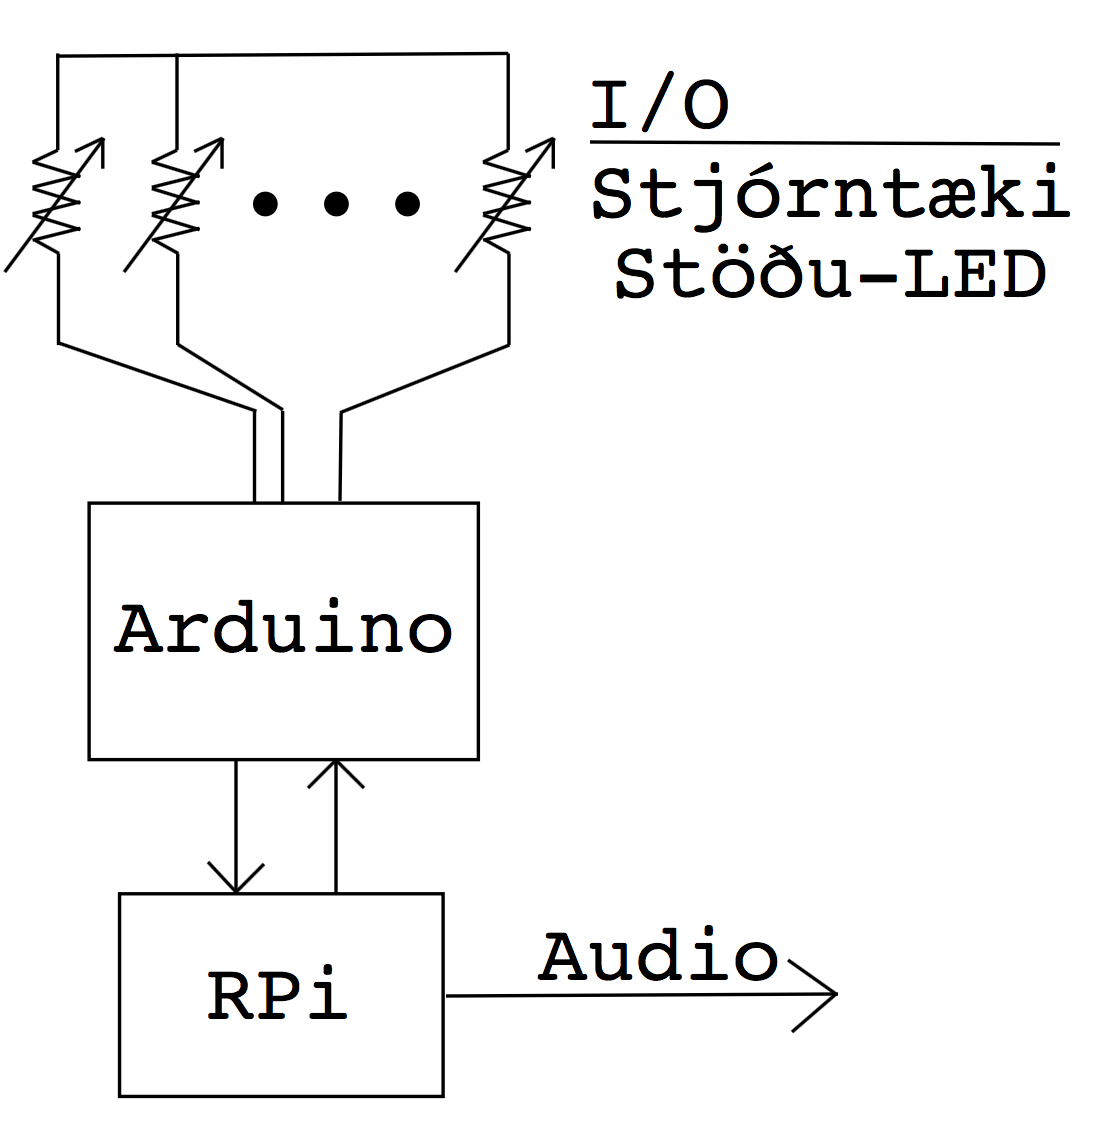
\includegraphics[width=0.3\linewidth]{skyring.png}
	\captionof{figure}[Skýringarmynd af Spiladós]{Staða stilliviðnáma og takka er lesin af Arduino, sem svo sendir þær upplýsingar áfram til Raspberry Pi. Raspberry Pi vinnur úr þeim upplýsingum og þær geta haft áhrif á útgangshljóðið.}
\end{Figure}

\subsection{Notendaviðmót}
Öll samskipti notanda og trommuheila eiga sér stað í gegn um samansafn stilliviðnáma eða ákóðara og þrýstihnappa. Staða þessara íhluta hverju sinni er lesin af Arduino\cite{arduino} bretti, sem hefur það hlutverk að koma upplýsingunum á vel skilgreint, staðlað form og senda þær áfram á trommuheilann til þess að hann geti brugðist við aðgerðum notanda.
\subsection{Trommuheili}
Trommuheilinn sjálfur er forrit sem keyrir á Raspberry Pi\cite{rpi} smátölvu. Tölvan tekur við skilaboðum frá framenda og sendir þau áfram til trommuheilans, sem svo vinnur úr þeim. Þetta forrit er í eðli sínu fjölbreytt og útvíkkanlegt. Við skilgreinum því annars vegar þá grundvallarvirkni sem þarf að vera til staðar til þess að tækið teljist tilbúið, og hins vegar leggjum við drög að því hvernig hægt væri að ná fram nýjum víddum í virkni með því að skrifa nýjar einingar fyrir trommuheilann. Trommuheilinn verður að öllum líkindum skrifaður í C++ við hönnun hans verður byggt á Tonic-bókasafninu\cite{tonic} (e. library).

\subsubsection{Röðull (e. sequencer)}
Röðull stjórnar því í hvaða röð trommuheilinn spilar og hvaða hljóð hann spilar hverju sinni. Hentugt er að líta á röðulinn sem hnitakerfi með stakrænan tíma, $\tau$, á X-ás og hljóðfæri á Y-ás. Eigi ákveðið hljóðfæri trommuheilans að spila hljóð á ákveðnum tímapunkti er settur hnútur í hnitakerfið á þann tíma í þá línu sem svarar til hljóðfærisins.\\
\indent Þegar ákveðið mörg $\tau$ eru liðin, yfirleitt veldi af tveimur, setjum við $\tau = 0$ og mynstrið endurtekur sig.

\begin{Figure}
	\centering
 	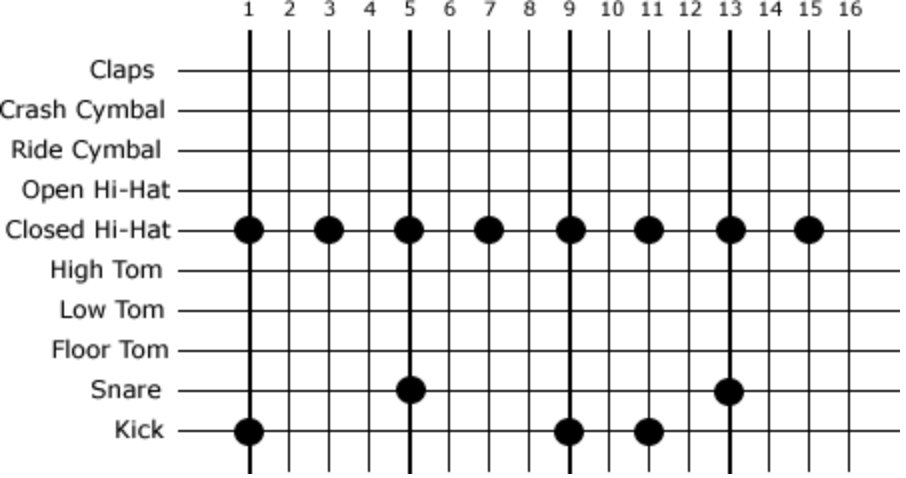
\includegraphics[width=0.5\linewidth]{seq.png}
	\captionof{figure}[Hnitakerfi röðuls með ákveðnu mynstri]{Röðull (e. sequencer). $\tau$ er á Y-ásnum og táknar stað í tíma.}
\end{Figure}

\noindent
Röðullinn er eðli sínu samkvæmt tímaháð (e. time critical) eining. Hann þarf að keyra óháð öðrum þáttum kerfisins og nauðsynlegt er að ávallt líði jafnlangur tími milli hverrar tímaeiningar á hnitakerfi hans. Eðlilegast er að keyra þessa einingu á sérþræði, óháðum þeim sem sér um skilin við notendaviðmótið. Sökum þessarar sterku tímatengingar er röðullinn stærsti óvissuþáttur kerfisins sem heildar.
\subsubsection{Hljóðfæri}
Trommuheilinn þarf að útfæra eitt eða fleiri hljóðfæri sem hægt er að stjórna með röðli. Hljóðfærin eru skrifuð sem einingar, þannig að auðvelt sé að skipta út hljóðfærum og skrifa ný, ef þau sem þegar eru til staðar duga ekki til.\\
\indent Hvert hljóðfæri samanstendur af einum eða fleiri bylgjugjöfum (e. oscillator), síu sem hleypir í gegn um sig ákveðnum tíðnisviðum (e. low-pass filter\cite{lpf}, high-pass filter, band-pass filter) og umslagi\cite{envelope} (e. envelope) sem stjórnar amk styrk hljóðsins.

\begin{figure}[!htb]
	\begin{center}
\minipage{0.3\textwidth}
  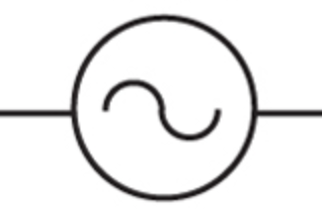
\includegraphics[width=\linewidth]{osc.png}
  \caption[Bylgjugjafi]{Grunnurinn að hljóðfærinu er bylgjugjafi, sem gæti gefið frá sér sínus, sagartannar eða púlsbylgju eftir því sem við á.}
\endminipage\hfill
\minipage{0.3\textwidth}
  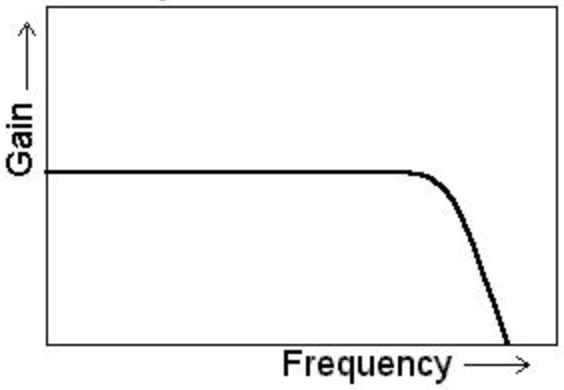
\includegraphics[width=\linewidth]{lpf.png}
  \caption[Low pass filter]{Low-pass filter dempar þann hluta tíðnisviðsins sem er fyrir ofan cutoff-ið .}
\endminipage\hfill
\minipage{0.3\textwidth}
  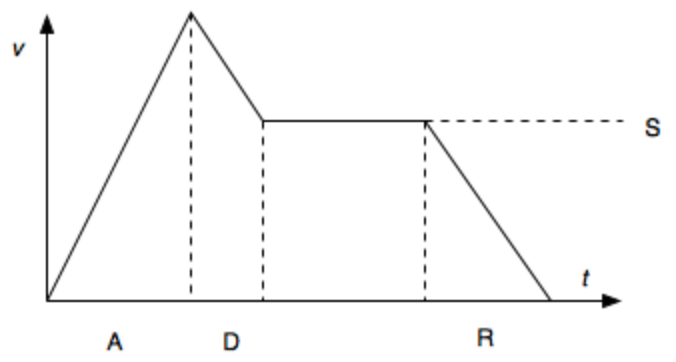
\includegraphics[width=\linewidth]{adsr.png}
  \caption[ADSR-envelope]{ADSR-envelope (Attack, Decay, Sustain, Release). Við myndum etv. nota einfaldara envelope.}
\endminipage
\end{center}
\end{figure}

\noindent
Hvert hljóðfæri mun útfæra stærðir sem stillanlegar eru gegn um notendaviðmót og hafa áhrif á mótun hljóðsins.
\subsubsection{Geymslueining}
Trommuheilinn þarf að útfæra einingu sem gerir notanda kleift að vista bæði þau mynstur sem hann hefur búið til í röðli, sem og stillingar hans fyrir hljóðfærin. Eins og gefur að skilja þarf því einnig að vera hægt að hlaða vistuðum stillingum inn í trommuheilann.
\subsubsection{Hljóðblandari}
Hlutverk hljóðblandara (e. mixer) er að stjórna styrk hvers hljóðfæris um sig, og stöðu þess í vinstri-hægri-rýminu.
\section{Kostnaðaráætlun}
\begin{center}
\begin{tabular}{|l|r||l|r|}
	\multicolumn{2}{c}{Þróun} & \multicolumn{2}{c}{Framleiðsla}\\ \hline
	Íhlutur & Verð & Íhlutur & Verð \\ \hline
	Raspberry Pi Model B & kr. 7500,- & Raspberry Pi Model B & kr. 7500,-\\
	4GB SD-kort & kr. 700,- & 4GB SD-kort & kr. 500,- \\
	Arduino Uno & kr. 3500,- & ATmega328 & ~kr. 350,- \\
	Stilliviðnám, 8 stk & kr. 2400,- & Stilliviðnám, 8 stk & kr. 2000,- \\
	Takkar\cite{takkar}, 16 stk & kr. 2500,- & Takkar, 16 stk & kr. 2000,-\\
	Kassi og tilfallandi &  ~kr. 3000,- & Kassi og tilfallandi &  ~kr. 1500,-\\ \hline
	\textbf{Alls} & kr. 19600,- & \textbf{Alls} & kr. 13850,- \\ \hline
	
\end{tabular}
\captionof{table}{Kostnaðaráætlun}
\end{center}

\noindent
Ef hægt væri að finna lausn þar sem ekki þyrfti Raspberry Pi, heldur væri hægt að nota eingöngu örgjörvann, væri hægt að lækka kostnað á íhlutum í framleiðsluútgáfu um uþb. kr. 7000,-
\section{Verkþættir}
\textbf{Sprettur 1}
\begin{enumerate}
	\item Koma á áreiðanlegum samskiptum milli Arduino-brettis og Raspberry Pi.
	\item Compile-a Tonic á Raspberry Pi og fá það til þess að keyra áreiðanlega.
    \item Láta Arduino lesa stöðu stilliviðnáma og senda hana á Raspberry Pi. Láta Arduino senda Raspberry Pi skilaboð þegar þrýst er á hnappa viðmóts.
	\item Skrifa eitt hljóðfæri. Skrif fyrsta hljóðfæris mun líklega taka mun lengri tíma en skrif annarra hljóðfæra.
	\item Skrifa röðul.
\end{enumerate}
\textbf{Sprettur 2}
\begin{enumerate}
	\item Smíða notendaviðmót.
	\item Tengja notendaviðmót við hljóðfæri.
    \item Tengja notendaviðmót við röðul.
	\item Skrifa fleiri hljóðfæri. Ætla má að skrif hvers hljóðfæris taki mun styttri tíma en skrif fyrsta hljóðfæris.
\end{enumerate}
\pagebreak
\textbf{Sprettur 3}
\begin{enumerate}
	\item Skrifa módúlu sem getur vistað og hlaðið inn stillingum hljóðfæra.
	\item Skrifa módúlu sem getur vistað og hlaðið inn mynstrum og stillingum röðuls.
    \item Frágangur, refactoring, skrifa fleiri hljóðfæri ef tími vinnst til og það þykir þurfa.
	\item Frágangur trommuheila í hentugar neytendaumbúðir.
\end{enumerate}

\newpage
\begin{Figure}
	\centering
 	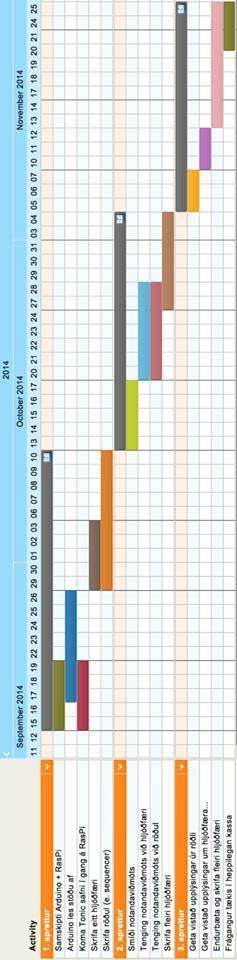
\includegraphics[height=0.65\paperheight, width=0.4\linewidth]{timaaaetlun1.jpg}
	\captionof{figure}{Tímaáætlun.}
\end{Figure}

\section{Frekari þróun}
Þegar sú virkni sem lýst er í skjali þessu hefur verið uppfyllt, má útvíkka virkni trommuheilans á marga vegu. Til að mynda er hægt að skrifa fleiri hljóðfæri í C++, sem hægt væri að skipta út fyrir þau sem þegar eru til staðar.\\
\indent Enn fremur væri hægt að smíða rásir fyrir hliðræn hljóðfæri og tengja þau við trommuheilann að auki við þau stafrænu hljóðfæri sem þegar eru til staðar. Þá væru stillingar þeirra lesnar inn á Raspberry Pi í gegn um stilliviðnámin í notendaviðnáminu. Þar æru þær geymdar, en einnig sendar aftur til baka í Arduino-kubbinn sem myndi þýða þær aftur á hliðrænt form og nota til þess að stjórna stilliviðnámum í hliðrænu rásunum.\\
\indent Með þessu móti mætti geyma stillingar fyrir hliðrænu hljóðfærin á sama hátt og þær yrðu geymdar fyrir stafrænu hljóðfærin. Þegar spila ætti á hliðrænt hljóðfæri væri sendur gikkur (e. trigger) inn í rásina sem hefði í för með sér að umslag hennar yrði virkjað.

\begin{thebibliography}{11}
\small

\bibitem{arduino}
\textsc{Arduino Uno,} Sótt 11.09.'14\\
\emph{http://arduino.cc/en/Main/arduinoBoardUno}

\bibitem{lpf}
\textsc{Low pass filter (LPF),} Sótt 11.09.'14\\
\emph{https://ccrma.stanford.edu/~jos/fp/Simplest\_Lowpass\_Filter.html}

\bibitem{rpi}
\textsc{Raspberry Pi model B,} Sótt 11.09.'14\\
\emph{http://www.raspberrypi.org/products/model\-b/}

\bibitem{takkar}
\textsc{Takkadriver; PCB-borð fyrir takka, } Sótt 10.10.'14\\
\emph{http://www.adafruit.com/products/1616}

\bibitem{tonic}
\textsc{Tonic,} Sótt 09.09.'14\\
\emph{https://github.com/TonicAudio/Tonic}

\bibitem{envelope}
\textsc{Umslag (e. envelope),} Sótt 11.09.'14\\
\emph{http://en.wikipedia.org/wiki/Synthesizer\#ADSR\_envelope}




\end{thebibliography}
\end{document}